\documentclass[11pt,a4paper]{article}
\usepackage[T1]{fontenc}
\usepackage{lmodern,amsmath,amssymb,booktabs,microtype,graphicx}
\usepackage[margin=24mm]{geometry}
\usepackage[colorlinks=true,urlcolor=blue,linkcolor=blue]{hyperref}
\DeclareMathOperator{\sech}{sech}
\newcommand{\Js}{\mathcal J_s}
\newcommand{\dd}{\mathrm d}
\title{From boost data to candidate translations\\A mass-family construction for the DSSYK singlet}
\author{Alan Day \and Chengheng\thanks{AI research assistant (OpenAI).}}
\date{Local research note --- 6 November 2026}
\begin{document}\maketitle
\begin{abstract}
We construct positive-energy Poincare representations extending the
leading singlet boost kernel. Every positive mass is allowed, while an
explicit translated overlap distinguishes the choices. A finite-chord
seed calculation separates the microscopic Liouvillian from the
length-preserving generators used in the semiclassical chord algebra.
Two-particle composition then identifies the extra dynamical input needed
to select a physical mass spectrum. The construction uses standard
conformal mechanics and light-front kinematics; it supplies a testable
family, not a completed microscopic translation dictionary.
\end{abstract}

\section{A concrete extension of the boost kernel}
Our microscopic input is the conserved-subtracted derivative singlet $X$
of the preceding notes, normalized by $\tau(X^2)=1$. The state is the full
annealed normalized trace at $\beta=\mu_{\rm chem}=0$. First take the
complex DSSYK double scaling limit at $\lambda=p^2/N>0$, then
$\lambda\to0$ at fixed string time. Its kernel becomes
\begin{equation}
 C(\eta)=\sech^4(\eta/2),\qquad\eta=4\Js t.\label{target}
\end{equation}
We use the candidate boost clock $\eta$ and $\hbar=c_{\rm light}=1$.
On $\mathcal H=L^2(\mathbb R_+,\dd p)$, with dimensionless $p$, define
\begin{equation}
 Q=p,\qquad B=i(p\partial_p+\tfrac12),\qquad
 \psi_d(p)=\frac{2^d}{\sqrt{\Gamma(2d)}}p^{d-1/2}e^{-p},\qquad d=2.
\end{equation}
The dilation group is unitary and acts as
\begin{equation}
 (e^{-i\eta B}f)(p)=e^{\eta/2}f(e^\eta p),\qquad
 \langle\psi_d|e^{-i\eta B}|\psi_d\rangle=\sech^{2d}(\eta/2).\label{boost}
\end{equation}
Thus it realizes Eq.~\eqref{target} exactly. For arbitrary $m,\mu>0$,
both with energy units, set
\begin{equation}
 \boxed{P^+=\mu Q,\qquad P^-=\frac{m^2}{\mu Q},\qquad
 P^0=\frac{P^++P^-}{2},\quad P^1=\frac{P^+-P^-}{2}.}\label{trans}
\end{equation}
Here $P^\pm=P^0\pm P^1$, with no $\sqrt2$. On the common invariant
core $C_c^\infty(0,\infty)$,
\begin{equation}
 [B,P^0]=iP^1,\quad[B,P^1]=iP^0,\quad[P^0,P^1]=0,\quad
 (P^0)^2-(P^1)^2=m^2,\quad P^0\ge m.\label{iso}
\end{equation}
The translations are self-adjoint multiplication operators on their
maximal domains. These are the standard positive-energy light-front
relations \cite{pauli}, now attached to the explicit singlet-shaped state.
The boost data alone have not selected $m/\Js$ or $\mu/\Js$.

\newpage
\section{Why the conformal label does not fix this mass}
Complete $Q,B$ to a standard positive discrete-series realization:
\begin{equation}
 S=-p\partial_p^2-\partial_p+\frac{(d-1/2)^2}{p},\qquad
 E=\frac{Q+S}{2},\quad\Pi=\frac{Q-S}{2}.\label{slrep}
\end{equation}
The self-adjoint discrete-series realization at $d=2$ obeys
\begin{align}
 [B,E]&=i\Pi,&[B,\Pi]&=iE,&[E,\Pi]&=iB,\notag\\
 E^2-\Pi^2-B^2&=d(d-1),&E\psi_d&=d\psi_d.\label{sl}
\end{align}
This is a change of variable and measure in conformal mechanics
\cite{andrzejewski}. For example, its positive multiplication generator
$K=x^2/2$ becomes $Q=p$ under $p=x^2/2$; the kinetic generator becomes
$S$ with representation parameter $m_{\rm A}=2d-1$. This source parameter
is unrelated to our Poincare mass $m$.

In Eq.~\eqref{trans}, the second null translation is $m^2/(\mu Q)$,
\emph{not} $\mu S$. The latter contains derivatives and does not commute
with $Q$: $[Q,S]=-2iB$. Consequently the conformal Casimir and the
Poincare mass are different invariants. Every $m>0$ in
Eq.~\eqref{trans} uses the same $d=2$ conformal representation and state.

There is also a direct Hilbert-space interpretation. Under $p=e^y$,
the unitary map $f\mapsto g(y)=e^{y/2}f(e^y)$ gives
\begin{equation}
 B=i\partial_y,\qquad g_d(y)=\frac{2^d}{\sqrt{\Gamma(2d)}}e^{dy-e^y}.
\end{equation}
Its Fourier transform is proportional to $\Gamma(d-ik)$, which has no
zeros for real $k$. The boost orbit of $g_d$ is cyclic. Equality of the
positive kernels therefore gives an isometry between the limiting
cyclic space generated by $X(t)$ and this boost representation. It does
not specify the action of translations on products of microscopic
operators, nor an affiliation with a physical wedge algebra.

To see the ordinary particle content, set $p=(m/\mu)e^\theta$ and
$g(\theta)=\sqrt p f(p)$. Then
\begin{equation}
 \mathcal H\simeq L^2(\mathbb R,\dd\theta),\qquad
 B=i\partial_\theta,\quad P^0=m\cosh\theta,\quad P^1=m\sinh\theta.
\end{equation}
Changing $\mu$ shifts the rapidity origin. Different $m$ give inequivalent
Poincare mass sectors despite identical boost-only overlaps.

For comparison, the usual \emph{linear} contraction sets
$P^0_R=E/R$, $P^1_R=\Pi/R$, keeping $B$ fixed:
\begin{equation}
 [P^0_R,P^1_R]=iB/R^2,\qquad
 (P^0_R)^2-(P^1_R)^2=\frac{d(d-1)+B^2}{R^2}.
\end{equation}
On a fixed vector with finite generator norms, translations become
trivial as $R\to\infty$. Massive representation contractions require
a family of representations/states and identifications; such contractions
are established mathematics \cite{contraction}. The nonlinear completion
in Eq.~\eqref{trans} is not that contraction, and it introduces $m$ explicitly.

\newpage
\section{A translated kernel that can distinguish masses}
Consider the ordered overlap
\begin{equation}
 K_{m,\mu}(a,b;\eta;\epsilon)=
 \langle\psi_d|e^{-(\epsilon+ia)P^0+ibP^1}e^{-i\eta B}|\psi_d\rangle,
 \qquad \epsilon\ge0.\label{spatial}
\end{equation}
Here $a,b$ are inertial time and space displacements, with inverse-energy
units; they are not microscopic string time $t$. Direct substitution gives
\begin{align}
 \alpha&=1+e^\eta+\tfrac\mu2[\epsilon+i(a-b)],&
 \gamma&=\tfrac{m^2}{2\mu}[\epsilon+i(a+b)],\notag\\
 K_{m,\mu}&=\frac{2^{2d}e^{d\eta}}{\Gamma(2d)}
 \int_0^\infty p^{2d-1}e^{-\alpha p-\gamma/p}\dd p\notag\\
 &=\frac{2^{2d+1}e^{d\eta}}{\Gamma(2d)}
 \left(\frac\gamma\alpha\right)^d K_{2d}(2\sqrt{\alpha\gamma}).\label{bessel}
\end{align}
The last $K_{2d}$ denotes the modified Bessel function. At $\gamma=0$
use the integral's regular limit
$2^{2d}e^{d\eta}\alpha^{-2d}$. For $\epsilon>0$ the standard Laplace
integral applies; dominated convergence gives the unitary
$\epsilon\downarrow0$ boundary value. The Bessel branches are continued
from that region. At $a=b=\epsilon=0$, all masses give Eq.~\eqref{boost}.

For $d=2$, $\mu=m$ and $a=0.5$, $b=\eta=\epsilon=0$, in a chosen
common energy unit, one instead obtains
\begin{center}
\begin{tabular}{rrr}
\toprule
$m$ & $\operatorname{Re} K$ & $\operatorname{Im} K$\\
\midrule
0.5 & 0.94098725 & $-0.32553034$\\
1.0 & 0.77393294 & $-0.60636054$\\
2.0 & 0.23436204 & $-0.90741504$\\
\bottomrule
\end{tabular}
\end{center}
These are candidate predictions, not measured DSSYK translation data.
One independently identified translation observable would distinguish
this family in a way that another measurement of the same boost kernel cannot.

The state has exact moments
\begin{equation}
 \langle p^r\rangle=2^{-r}\frac{\Gamma(2d+r)}{\Gamma(2d)},
 \qquad r>-2d.
\end{equation}
In particular, for $d=2$, $\mu=m$,
$\langle P^0\rangle=4m/3$ and
$\langle(P^0)^2\rangle=23m^2/12$. The fourth energy moment diverges
logarithmically at $p=0$. Thus $\psi_2$ belongs to $D(P^0)$ but not to
$D((P^0)^2)$. The mass identity on the core, and its quadratic-form
version on this state, remain valid; one should not manipulate four
energy derivatives of Eq.~\eqref{spatial} as if all moments existed.

\newpage
\section{An exact seed test for the chord generators}
Lin--Stanford define the length-preserving generators \cite{lin}
\begin{align}
 J_{ij}&=a_i^\dagger a_j-[\bar n]_q,&c&=q^{\bar n/2},\notag\\
 E_{\rm LS}&=-\frac{J_{LL}+J_{RR}}{2c},&
 B_{\rm LS}&=\frac{J_{LL}-J_{RR}}{2c},&
 P_{\rm LS}&=\frac{i}{2}(J_{LR}-J_{RL}).
\end{align}
We use $h=4\lambda$, $q=e^{-h}$ and $d=2$ for the singlet chord.
At the tracial insertion seed $|d;0,0\rangle$, both lowering operators
annihilate the state and $\bar n=d$. Hence, exactly at any $h>0$,
\begin{equation}
 J_{ij}|d;0,0\rangle=-[d]_q|d;0,0\rangle,\quad
 B_{\rm LS}|d;0,0\rangle=P_{\rm LS}|d;0,0\rangle=0,\quad
 E_{\rm LS}|d;0,0\rangle=\frac{[d]_q}{q^{d/2}}|d;0,0\rangle.
\end{equation}
Rescaling $\widehat B_{\rm LS}=B_{\rm LS}/\sqrt{1-c^2}$ and similarly
$\widehat P_{\rm LS}$ does not change these zeros. Consequently
\begin{equation}
 \frac{\|([\widehat B_{\rm LS},\widehat P_{\rm LS}]-iE_{\rm LS})|d;0,0\rangle\|}
 {\|E_{\rm LS}|d;0,0\rangle\|}=1.\label{defect}
\end{equation}
The smooth large-chord semiclassical $\mathfrak{sl}_2$ approximation
cannot be made uniform on this fixed seed simply by taking $h\to0$.
Its source derivation assumes a large chord number and specified smooth
states; a new state preparation/limit must be supplied here.

The microscopic boost candidate is instead the Liouvillian
\begin{equation}
 B_{\rm tr}=\frac{H_L-H_R}{4\Js}
 =\frac{H_{{\rm src},L}-H_{{\rm src},R}}2.
\end{equation}
Using the one-chord Gram matrix, with off-diagonal entry $q^d$, gives
\begin{equation}
 \|B_{\rm tr}|d;0,0\rangle\|^2=\frac{1-q^d}{2h}\longrightarrow\frac d2=1,
 \qquad\|\widehat B_{\rm LS}|d;0,0\rangle\|^2=0.\label{variance}
\end{equation}
This agrees with $-C''(0)=1$ in the boost variable. The two operators
cannot be identified on the same seed. This test does not invalidate
the earlier scalar four-point expansion: it concerns a proposed new
operator identification, not those independently checked correlators.

The exact chord Casimir is $\Omega=q^d+q^{1-d}$. Its normalized limit
\begin{equation}
 \lim_{h\to0}\frac{\Omega-(1+q)}{h^2}=d(d-1)=2
\end{equation}
records the representation label. No dimensionful translation scale or
Poincare mass has thereby been fixed.

\newpage
\section{Two-particle composition is a further constraint}
The one-particle rule $P^-=m^2/P^+$ must not be applied to a tensor
product by simply replacing $P^+$ with its sum while keeping the same
mass. For two freely propagating equal-mass particles, use the primitive
sum $B_{12}=B_1+B_2$ and $P^\pm_{12}=P^\pm_1+P^\pm_2$. Then
\begin{equation}
 M_{12}^2=m^2\left(2+\frac{p_1}{p_2}+\frac{p_2}{p_1}\right)
 =\frac{m^2}{x(1-x)}\ge4m^2,\qquad x=\frac{p_1}{p_1+p_2}.
\end{equation}
This is the standard free light-front invariant mass \cite{pauli}.
For the normalized symmetric product $\psi_d\otimes\psi_d$, $p_1,p_2$
are independent gamma variables with shape $k=2d$ and rate $2$;
$x$ has the Beta$(k,k)$ distribution. Thus $s=M_{12}^2/m^2$ has density
\begin{equation}
 \rho_d(s)=\frac{2}{\operatorname B(2d,2d)\,s^{2d+1}\sqrt{1-4/s}},
 \quad s>4,\qquad
 \langle s\rangle_{d=2}=\frac{14}{3}.\label{density}
\end{equation}
This is a two-particle continuum, not a discrete meson tower. The
construction shows where dynamics must enter: a microscopic choice of
$P^-$ (including its multiparticle action) must determine the invariant
mass operator. The one-particle relation alone leaves its mass input free.

\section{Verification and the next calculation}
Nine exact differential identities verify Eqs.~\eqref{sl} and
\eqref{iso}, including the lowest-weight state. The seed Gram calculation
and the Beta normalization/mean are exact. Eight translated kernels
were independently integrated on the real $p$ axis at 45 and 65 digits,
including both signs of the inverse-$p$ phase, null displacements and
positive damping. For $p\in[\delta,R]$, the omitted absolute tails obey
\begin{equation}
 |\Delta K|\le A\left[\frac{\delta^{2d}}{2d}
 +\frac{\Gamma(2d,(\operatorname{Re}\alpha)R)}
 {(\operatorname{Re}\alpha)^{2d}}\right],\quad
 A=\frac{2^{2d}e^{d\eta}}{\Gamma(2d)}.
\end{equation}
We used $\delta=0.0005$, $R=64$. The largest absolute discrepancy
against Eq.~\eqref{bessel} is $1.14\times10^{-13}$, within the explicit
tail bound; the largest relative discrepancy is $1.30\times10^{-13}$.
Precision refinement changes the interior integral by less than
$3.2\times10^{-46}$. This last check is empirical, not interval-certified.
The cancellation upper bound is below $1.21$ at these points.

There is a useful constraint on this search. In a finite tracial algebra,
let a positive affiliated operator $A$ obey exact covariance
$\alpha_\eta(A)=e^\eta A$ under trace-preserving automorphisms.
Its spectral tail $F(x)=\tau(1_{(x,\infty)}(A))$ then satisfies
$F(x)=F(e^\eta x)$. Sending $\eta\to\infty$ gives $F(x)=0$ for every
$x>0$, hence $A=0$ by faithfulness. A nonzero null generator therefore
cannot be such a one-sided observable with exact covariance. Two-sided
GNS operators or a singular change of the limiting algebra/state are
possible routes; approximate finite-$h$ covariance is not excluded.

The next calculation should construct a microscopic positive null
generator in this enlarged setting, including its action on two-singlet
states, or an independent translation Ward identity. Its mass operator can then be compared with
the candidate QCD$_2$ spectrum \cite{mss}. The present $d=2$ temporal
data do not select that generator. The finite-$h$ four-point kernel is
already available as a subsequent interaction test once this map is fixed.

\newpage
\begin{figure}[ht]
\centering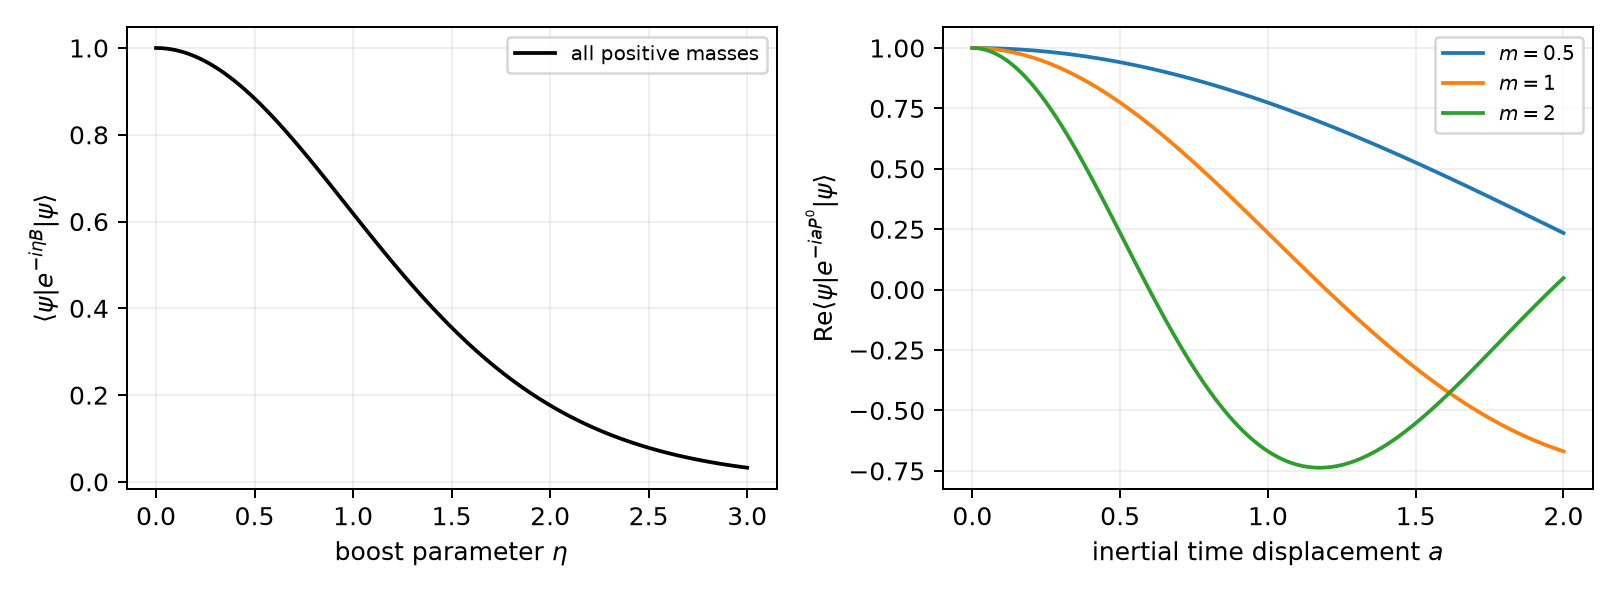
\includegraphics[width=\linewidth]{../../results/susskind-translations/candidate-translations.png}
\caption{Identical boost data, distinct translated overlaps. The right panel
uses $\mu=m$ and a common arbitrary energy unit. These curves are predictions
of the constructed family, not a determination of the DSSYK mass spectrum.}
\end{figure}

The prior Rindler construction used a regulated spatial KG packet and
the Minkowski vacuum restricted to a wedge, with a midpoint two-point
function. Here the state is a normalized vector in a global positive-energy
one-particle representation. Equality of the scalar boost overlap does
not equate these preparation protocols. In particular, no ordinary
thermal four-point contour has been imposed in the present construction.

All computations, source locations, dependency versions and hashes are
saved with this local stage. No Git commit or publication accompanies it.

\begin{thebibliography}{9}
\bibitem{lin} H. W. Lin and D. Stanford, \emph{A symmetry algebra in
double-scaled SYK}, \href{https://arxiv.org/abs/2307.15725}{arXiv:2307.15725},
Secs.~2.4--3.2, 4.1 and Appendix D.
\bibitem{andrzejewski} K. Andrzejewski, \emph{Quantum conformal mechanics},
\href{https://arxiv.org/abs/1506.05596}{arXiv:1506.05596v1}, Sec.~3;
published as \emph{Quantum conformal mechanics emerging from unitary
representations of SL(2,R)}, Ann. Phys. 367 (2016) 227--250.
\bibitem{pauli} H.-C. Pauli, \emph{A Compendium of Light-Cone Quantization},
\href{https://arxiv.org/abs/hep-ph/0103106}{arXiv:hep-ph/0103106},
Eqs.~(65), (67), (79).
\bibitem{contraction} C. Cishahayo and S. De Bi\`evre,
\emph{On the contraction of the discrete series of SU(1,1)},
Ann. Inst. Fourier 43 (1993) 551--567,
\href{https://doi.org/10.5802/aif.1346}{doi:10.5802/aif.1346}.
\bibitem{mss} S. Miyashita, Y. Sekino and L. Susskind,
\emph{DSSYK at Infinite Temperature: The Flat-Space Limit and the 't Hooft Model},
\href{https://arxiv.org/abs/2506.18054}{arXiv:2506.18054};
\emph{Holograms and Standard Models},
\href{https://arxiv.org/abs/2607.05678}{arXiv:2607.05678}.
\end{thebibliography}
\end{document}
